\documentclass[conference]{IEEEtran}


  	\usepackage[pdftex]{graphicx}
  	\graphicspath{{../pdf/}{../jpeg/}}
	\DeclareGraphicsExtensions{.pdf,.jpeg,.png}

	\usepackage[cmex10]{amsmath}
	\usepackage{mathabx}
	\usepackage[utf8]{inputenc}
	\usepackage{algorithmic}
	\usepackage{array}
	\usepackage{mdwmath}
	\usepackage{mdwtab}
	\usepackage{eqparbox}
	\usepackage{url}
	\usepackage{booktabs}
    \usepackage{lipsum}
	\usepackage{fouriernc}
	\usepackage{multirow, booktabs}
	\usepackage{pgfplots}
	\usepackage{float}
	\restylefloat{table}
	\hyphenation{op-tical net-works semi-conduc-tor}

\begin{document}

\title{\LARGE Análises de Sentimentos: abordagem lexical de classificação de opinião no contexto mercado financeiro brasileiro}

% \author{\authorblockN{Leave Author List blank for your IMS2013 Summary (initial) submission.\\ IMS2013 will be rigorously enforcing the new double-blind reviewing requirements.}
% \authorblockA{\authorrefmark{1}Leave Affiliation List blank for your Summary (initial) submission}}

 \author{\authorblockN{V. Peres\authorrefmark{1}, R. Vieira\authorrefmark{2}}
 \authorblockA{\authorrefmark{1}Pontifícia Universidade Católica do Rio Grande do Sul, Brasil \\vitor.peres@acad.pucrs.br}
 \authorblockA{\authorrefmark{2}Pontifícia Universidade Católica do Rio Grande do Sul, Brasil\\renata.vieira@pucrs.br}}

\maketitle

\begin{abstract}
Financial news and Specialist Opinion bring us the latest information about stock market. Some studies have shown how information can be useful if it is analyzed correctly. Extracting sentiments and opinions from specifics texts, can be a way of assisting in decision-making. In this paper, we present a sentiment analyser for financial texts using lexicon-based approach, in portuguese. Using polarity lexicon, we can identify the positive or negative polarity of each term in the corpus. And also, we build a lexicon with a specific corpus from TradingView website.
\end{abstract}

\IEEEoverridecommandlockouts
\begin{keywords}
Sentimental Analysis, Bag-Of-Words, Lexicon, Precision, TF-IDF, Polarity, OpLexicon, Sentilex
\end{keywords}

\IEEEpeerreviewmaketitle


% ===================
% # I. Introduction #
% ===================

\section{Introdução}

Com o aumento da informação gerada a partir de engajamento de usuários, vêm se observando a necessidade de gerar valor deste tipo de informação. No mercado financeiro não ocorre de maneira diferente, já que muitos dos investimentos passam por análises de especialistas com o objetivo de chegar a um senso comum de melhor opção. 

Neste sentido, investidores que estão no inicio de carreira procuram por opiniões que transmitem as melhores ideias de investimento. Através da análise de sentimentos é possível coletar qual o sentido da informação, categorizando-a em positiva ou negativa. Grande parte das aplicações que envolvem análises de sentimentos, vêm sendo direcionadas na análise de opiniões de produtos, onde o engajamento de consumidores servem de métrica para validar possíveis riscos e problemas \cite{Shahana:2015}. 

Neste trabalho será apresentado a abordagem de análise de sentimentos utilizando dicionários léxicos no contexto financeiro. O objetivo deste trabalho será avaliar diferentes léxicos e qual a sua performance para textos de domínio específico. E por fim, a criação de um léxico de domínio financeiro, a partir de um corpus de opiniões de investidores disponível na ferramenta TradingView. 

Na seção \ref{sec:dois} será apresentado a revisão literária em relação a analise de sentimentos. Na Sessão III, será apresentada o contexto e descrição dos dados deste trabalho. Na sessão IV será apresentado o modelo desenvolvido. Na sessão V serão apresentadas as etapas da construção do dicionário léxico. Seção VI os experimentos e resultados desta análise e por fim na seção VII a conclusão do trabalhos e as etapas futuras. 

% =======================================================
% # II. Revisão de Literatura                           #
% =======================================================

\section{\label{sec:dois}Revisão de Literatura}

Mizumoto \cite{Mizumoto:2012} propõe um estudo para determinar a polaridade de sentimentos em textos de noticias sobre mercado financeiro, utilizando dicionários léxicos. Além da construção de um dicionário léxico, fazendo o uso de aprendizado semi-supervisado, anotando manualmente a polaridade de um determinado numero de termos/palavras dos textos destas notícias. Ao final do estudo são comparados as polaridades determinadas pelo método proposta com as polaridade determinadas por especialistas de mercado financeiro. 

San \cite{Li:2013} também utiliza a abordagem léxica para a análise de sentimentos em notícias do mercado financeiro, sendo o mesmo feito sobre dois conjuntos de experimentos, que utilizam, ou não, o processo de stemming. 

Palanisamy \cite{palanisamy:2013} através de léxicos, procuram-se identificar qual tipo de sentimento de tweets que contenham variações de palavras, emoticons e hashtags. Em \cite{Devitt:2007}, o autor propõe o emprego de coesão léxica baseada em textos, na detecção de sentimentos e polaridade de textos.

% =============================================
% # III. Contexto e Descrição de Dados        #
% =============================================

\section{Contexto e Descrição de Dados}

Com o aumento de pessoas investindo no mercado de ações, é possível observar que muitas delas ainda não possuem conhecimento total da movimentação dos preços das ações nos gráficos. Com isso o mercado acaba pagando, pois muitas ações acabam perdendo volume\footnote{Volume representa o nível de atividade do mercado, sendo o motor que empurra e sustenta os movimentos dos preços. Baixo volume demonstra baixa participação dos investidores, e portanto pequeno comprometimento financeiro com o movimento em si, tornando-se frágil. Alto volume demonstra que os investidores estão atentos e ativos, oferecendo sustentação e validade aos movimentos aos sinais que percebemos \cite{ANALISETECNICA}} por falta de negociadores ou até mesmo pela falta conhecimento para manejar ações ditas desinteressantes.

\subsection{Base de Dados}

Foram coletadas para este estudo, um série de dados que contemplam 3 fontes diferentes. Dessas 3 fontes podemos citar: \textbf{Trading View}, ferramenta que possibilita operar no mercado financeiro com auxílio da comunidade trader, e melhorar o desempenho a partir da observação de outros traders. A \textbf{InfoMoney} é o maior site especializado em investimentos pessoais e educação financeira do Brasil, que fornece aos leitores informações que valem dinheiro de uma forma simples e agradável de ler. E por fim a \textbf{Investing.com} que é um portal financeiro global de dados e uma marca composta por 30 edições em 23 idiomas. Cada edição abrange uma ampla variedade de veículos financeiros locais e globais, incluindo ações, título públicos, commodities, câmbio, criptomoedas, taxas de juros, futuros e fundos. A coleta de dados para a análise contém ao total 2024 textos. A base do TradingView, consiste de uma base de 615 textos, dentre esses dados, temos 180 que não possuem rótulos e 435 textos com rótulos, estes que são definidos pelo usuário da plataforma em 3 categorias; \textit{Viés de Alta}, \textit{Viés de Baixa} e \textit{Educação}. InfoMoney e Investing.com, possuem 1309 e 100 textos, respectivamente.

\begin{table}
\caption{Textos e Rótulos Trading View} \label{tab:long} 
\centering
\begin{tabular}{>{\centering\arraybackslash}m{5.5cm}|>{\centering\arraybackslash}m{2cm}}
\hline
\hline
TEXTO & RÓTULO \\ \hline
Lucro da empresa ligado ao preço do petróleo e dólar . Dólar nos patamares de R\$ 4,10 força a dívida da empresa para cima. & Viés de Baixa \\ \hline
GOLL4 passou por recente período de correção, e gora retoma sua tendência de alta, confirmada pela mudança de status do indicador HILO e maior volume. Possibilidade de upside de 38\% aproximadamente. & Viés de Alta  \\ \hline
GGBR4 esta em um canal de alta e formou uma congestão em retângulo na metade do canal, depois de uma perna de alta.  Os preços tendem a atingir o topo do canal & Educação \\ \hline
\end{tabular}
\end{table}

% =============================================
% # IV. Modelo para Análise de Sentimentos    #
% =============================================

\section{Modelo para Análise de Sentimentos}

\begin{figure*}[h]
\begin{center}
% \fbox{\rule{0pt}{2in} \rule{.9\linewidth}{0pt}}
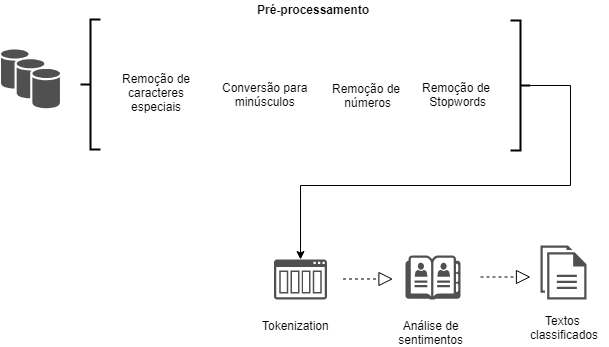
\includegraphics[width=0.6\linewidth]{DiagramaSentimenal.png}
\end{center}
   \caption{Modelo proposto para análise e classificação de sentimentos.}
\label{fig:bubble}
\end{figure*}

\subsection{Pré-processamento de Dados}

Para uma melhor performance do algoritmo criado, houve a necessidade de realizar a limpeza dos dados, que possibilita através de abordagem de dicionario léxico percorrer as sentenças de maneira simples. Esse processo têm sido aplicado a textos que não possuem a estrutura formal, no caso textos de Twitter, e contem uma serie de significativas de ruídos \cite{Symeon:2018}. Estes que pela definição, se caracterizam por dados que não entregam informação útil para análise em questão.

\begin{itemize}
    \item \textit{Remoção Caracteres Especiais}: caracteres especiais, que dentro deste contexto, como quebra de linhas, url's e cifrões não geram valor na análise e sua retirada em eminente; 
    \item \textit{Conversão para Minúsculos}: o processo de conversão do texto para minusculo, melhora a combinação de palavras e reduz o problema de dimensionalidade \cite{Santos:2014};
    \item \textit{Remoção de Números e Pontuações}: a presença de pontuação em alguns casos, denota a existência de algum tipo de sentimento. No caso de uma frase que tem seu termino com uma \textit{exclamação}, pode induzir a um sentido de intensidade positiva ou negativa. O mesmo vale para números, que indicam quantidade de determinado termo e não indicam sentimento \cite{He:2011};
    \item \textit{Remoção StopWords}: as StopWords são palavras que possuem alta frequência nas sentenças, e não contém valores úteis dentro da análise. São classificadas como StopWords preposições, artigos, conjunções e dentre outros. Nesta análise, foi feito o uso do pacote NLTK de StopWords em português \cite{Loper:2002}. 
\end{itemize}

\subsection{Polaridade de Textos}

A classificação dos textos parte de uma comparação das sentenças (textos) com as palavras disponíveis no léxico. Após a fase de pré-processamento cada sentença é \textit{Tokenizada}, processo que separa em objetos únicos os termos presentes na string, facilitando a análise por parte do algoritmo \cite{Taweh:2018}. 

A partir desta etapa, são comparadas cada objeto único das strings com os termos disponíveis em cada léxico. A cada palavra encontrada, é adiciona a uma lista temporária os valores referentes a positivo (1) e negativo (-1), e caso não haja o termo a comparar no léxico é adicionado o valor neutro (0). Após, somas são realizadas para concretizar a polaridade dos textos, conforme a fórmula a seguir:

\begin{equation*}
    \sum_{k=1}^{N} t(i,j)
\end{equation*}

Onde \textit{t(i, j)} representa a palavra/termo (i) e sua polaridade (j) de acordo com a sua disponibilidade no léxico. Realizado somatório dos termos de uma sentença, são analisados em qual pesos devem ser classificados. Por exemplo, um texto tem como resultado do seu somatório o valor de 4, visto nossa caracterização anterior de termos, classificamos a polaridade de textos da seguinte maneira: 

\begin{table}[H]
\caption{Tipos de Classificação} \label{tab:long} 
\centering
\begin{tabular}{|c|c|}
\hline
Valor Somatório & Classe \\ \hline
menor que -2 & Muito Negativo \\ 
entre -0.5 e -1 & Negativo \\ 
entre -0.5 e 0.5 & Neutro \\ 
entre 0.5 e 1 & Positivo \\ 
maior que 1 & Muito Positivo \\ \hline
\end{tabular}
\end{table}

\subsection{Abordagem Lexical}

\subsubsection{OpLexicon}

O OpLexicon, construído a partir do estudo de Souza \cite{Souza:2011}, consiste de uma aplicação de 3 técnicas diferentes presentes na literatura: \textit{Turney's Corpus-based}, \textit{Thesaurus-based} e uma variação de \textit{Mihalcea}, utilizando um sistema de tradução automática. 

O corpus utilizado no estudo é composto por 346 reviews de filmes em português brasileiro, extraídos do site CinePlayers e Cinema com Rapadura, e de 970 textos jornalísticos sobre diferentes temas extraídos do PLN-Br Categ corpus. TEP Thesaurus foi utilizado como recurso léxico dentro do estudo, este que contém 44077 palavras e anotações de synsets e antônimos. 

\subsubsection{SentiLex}

Constitui de 6321 lemmas e 25406 formas flexionadas. Os atributos de cada entrada do léxico são: a polaridade do adjetivo, algo do sentimento e método de atribuição de polaridade. 

\subsubsection{UniLex}

UniLex foi construído a partir de um corpus extraído do twitter, sobre o tema política, rotulados e comparados para a criação do léxico. 

\section{Construção de Dicionário Léxico}

Verificado a disponibilidade de dados rotulados (TradingView), observou-se a possibilidade da criação de um léxico especifico em mercado financeiro. Como mencionado anteriormente, o dataset extraído da ferramenta TradingView, contém a classificação do texto inserida manualmente pelo usuário. 

\subsection{Bag Of Words}

A essência deste técnica é converter documentos de textos em vetores, de modo que cada documento seja convertido em um vetor que represente a frequência de todas as palavras distintas presentes em um espaço vetorial de um documento \cite{Dipanjan:2016}.  

\begin{figure*}[h]
\begin{center}
% \fbox{\rule{0pt}{2in} \rule{.9\linewidth}{0pt}}
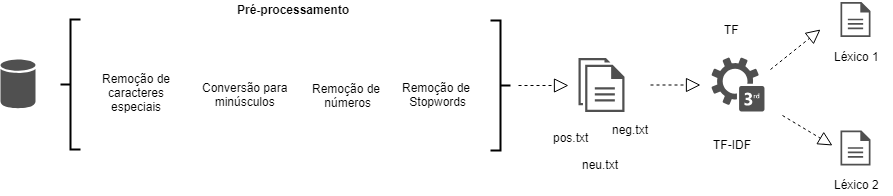
\includegraphics[width=0.6\linewidth]{Lexicon.png}
\end{center}
   \caption{Modelo Construção do Léxico.}
\label{fig:lex}
\end{figure*}

\subsection{TF-IDF}

Abreviação do termos \textit{Term Frequency-inverse Document Frequency}, que indica a ponderação de termos que ocorrem em termos proporcionalmente à sua frequência. Esta técnica foi originalmente desenvolvida como uma métrica para funções de classificação, na busca de resultados em mecanismos de busca, baseadas em consultas de usuários. 

\begin{equation*}
    W_t_,_d = \left ( \frac{Freq_t_,_d}{Max} \right ) * log_2 \left ( \frac{N}{n_t} \right)
\end{equation*}

Onde \( W_t_,_d \) é o peso de termo \textit{t} no documento \textit{d}. \( Freq_t_,_d \) é q quantidade de vezes que o termo/palavra ocorre em um texto. \( Max \) é o termo que possui maior ocorrência no texto. \( N \) é o total de textos na base de testes, \( n_t \) é o número de textos na base de testes que possui o termo \( t \).

\section{Experimentos e Resultados}

Neste trabalho iniciamos os experimentos utilizando o modelo anteriormente descrito, nos 3 conjuntos de dados: \textit{TradingView, Investing.com e InfoMoney}. Inicialmente foi realizado os experimentos se nenhum tipo de tratamento dos dados, e assim foi observado métricas fora do normal. Então novamente, verificou o estado da arte e verificado quais seriam as etapas fundamentais para um melhor resultado, com os mesmos presentes na tabela \ref{T:equipos}. 

Com o objetivo de avaliar o modo que o algoritmo esta classificando os textos, foi definido a utilização das métricas Precision, Recall, F1-score e Acuracy, bastante utilizando em algoritmos de classificação supervisionada. Neste etapa, utilizaremos o conjunto de dados do TradingView, que do montante total de 615 textos, apenas 435 são rotulados. Estes sendo 286 positivos, 19 neutros e 130 negativos. 

\begin{table}[H]
    \caption{Performance do Algoritmo Léxico} \label{tab:perf} 
    \centering
    \begin{tabular}{|c|c|c|}
    \hline
    Métrica & OpLexicon & SentiLex \\ \hline
    Precision & 0,693 & 0,721 \\ 
    Recall & 0,763 & 0,822 \\ 
    F1-score & 0,725 & 0,76 \\ 
    Acuracy & 0,6 & 0,673 \\ \hline
    \end{tabular}
\end{table}

\begin{table*}[h]
    \caption{Resultados das análises de sentimentos por léxico.} \label{tab:long} 
    \label{T:equipos}
    \begin{center}
        \begin{tabular}{| c | c | c | c | c | c | c |} \hline
             & \multicolumn{3}{ c |}{\textbf{SentiLex}} & \multicolumn{3}{ c |}{\textbf{OpLexicon}}\\ 
            \cline{0-7}
            & \textbf{POS} & \textbf{NEU} & \textbf{NEG} & \textbf{POS} & \textbf{NEU} & \textbf{NEG} \\ \hline  
            InfoMoney       & 174 & 999 & 135 & 343 & 649 & 316 \\ \hline
            Investing.com   & 5 & 86 & 9 & 17 & 60 & 23 \\ \hline
            TradingView     & 220 & 157 & 71 & 390 & 112 & 124 \\ \hline
            \end{tabular}
    \end{center}
\end{table*}

% \begin{table*}[h]
%     \caption{Resultados das análises de sentimentos por léxico.} \label{tab:long} 
%     \label{T:equipos}
%     \begin{center}
%         \begin{tabular}{| c | c | c | c | c | c | c | c | c | c |} \hline
%              & \multicolumn{3}{ c |}{\textbf{SentiLex}} & \multicolumn{3}{ c |}{\textbf{OpLexicon}} & \multicolumn{3}{ c |}{\textbf{UniLex}} \\ 
%             \cline{0-10}
%             & \textbf{POS} & \textbf{NEU} & \textbf{NEG} & \textbf{POS} & \textbf{NEU} & \textbf{NEG} & \textbf{POS} & \textbf{NEU} & \textbf{NEG} \\ \hline  
%             InfoMoney       & 174 & 999 & 135 & 343 & 649 & 316 & 531 & 247 & 527 \\ \hline
%             Investing.com   & 5 & 86 & 9 & 17 & 60 & 23 & 40 & 27 & 32 \\ \hline
%             TradingView     & 220 & 157 & 71 & 390 & 112 & 124 & 388 & 49 & 195 \\ \hline
%             \end{tabular}
%     \end{center}
% \end{table*}

Dentre os léxicos que melhor obtiveram acurácia podemos notar que o SentiLex chegou a \textbf{0.673} contra \textbf{0.6} do OpLexicon. Também vale ressaltar que nas outras métricas de Recall, Precision e F1-score, SentiLex teve pequena vantagem em relação ao OpLexicon (tabela \ref{tab:perf}). Feita esta análise, partimos agora para a construção de um léxico, este que foi baseado na técnica TF-IDF, definida na seção anterior. 

O processo de construção inicia no pré-processamento de dados, e na divisão do dataset em arquivos de acordo com sua classificação prévia (Figura \ref{fig:lex}). O uso de \textit{Bag of Words} ajuda na conversão de documentos em vetores, e facilita a manipulação dos mesmos, além de possibilitar a geração da frequência do aparecimento de palavras. De cada arquivo separado, foram indicados a frequência assim como sua polaridade.

\begin{itemize}
    \item \textbf{Positivo}: "\textit{Alta, Queda, Oportunidade, Rompendo}";
    \item \textbf{Neutro}: "\textit{Força, Retração, Romper, Risco, Queda}";
    \item \textbf{Negativo}: "\textit{Vermelho, Resistência, Negativo}".
\end{itemize}

Fica evidente que apenas calcular a frequência de palavras pode não ser a melhor opção, sendo assim optamos por verificar o mesmo processo, porem com a aplicação da técnica TF-IDF. Isso também é um estimulo já que muitas das palavras se repetiam com polaridades diferentes. 

\begin{itemize}
    \item \textbf{Positivo}: "\textit{Acumular, Reagiu, Caiu, Disparando}";
    \item \textbf{Neutro}: "\textit{Ideal, Sustentado, Margem, Correção, Gerou}";
    \item \textbf{Negativo}: "\textit{Revertendo, Falha, Difícil}".
\end{itemize}

Com o uso de TF-IDF verificou-se alguns termos que no significado real da palavra, estariam relacionados ao sentimento contrario. Por exemplo, foram classificados como positivos os termos \textbf{Reagiu} e \textbf{Caiu}, que no contexto financeiro, o termo "reagiu" pode estar relacionado a uma opção de investimento que não fosse trazer grande lucro, e o termo "caiu", à um acontecimento que pode gerar lucro devido a sua variação de preço. 

% ==================
% # IV. CONCLUSÃO  #
% ==================

\section{Conclusão}

Este trabalho apresentou o uso de dicionários léxicos, com o objetivo de classificar textos específicos sobre o mercado financeiro. Além de verificar o quão próximo um léxico pode classificar textos já classificados. 

Dos experimentos realizados, verificamos que o SentiLex conseguiu obter o melhor resultado comparado com o OpLexicon, tendo como resultado de precisão mais de 70\%. Já o processo de construção de um léxico, foi analisado duas abordagens, sendo a ultima, utilizando TF-IDF, a que melhor se aproximou dos termos que o mercado de ações contem. 

Como trabalhos e extensões futuras desta pesquisa, é citada a possibilidade de comparação de algoritmos supervisionados como NaiveBayes, SVM e dentre outros, com a abordagem léxica. Outra possibilidade, é a inclusão de mais técnicas de pré-processamento de dados, como por exemplo o uso de Stemming e Normalização de textos, que podem ainda assim influenciar em melhores resultados. E na construção do léxico, a inserção de Part-of-Speach nos termos, isso sendo possível através da integração com outros léxicos mais completos, como a WordNet por exemplo. Além de inserir as variações gramaticais das palavras, utilizando a técnica stemming de maneira reserva. Ao inserir stemming em uma palavra, será extraído o seu radical, assim é possível combinar com os termos que a WordNet possui, da maneira a enriquecer o léxico. 

% ==================
% # ACKNOLEDGMENTS #
% ==================

% use section* for acknowledgement
%\section*{Acknowledgment}
% The authors would like to thank...


% ==============
% # REFERENCES #
% ==============

\bibliographystyle{IEEEtran}
\bibliography{IEEEabrv,biblio_traps_dynamics}

\end{document}
